%%%%%%%%%%%%%%%%%%%%%%%%%%%%%%%%%%%%%%%%%%%%%%%%%%%
%                                                 %
%                     SECTION                     %
%                                                 %
%%%%%%%%%%%%%%%%%%%%%%%%%%%%%%%%%%%%%%%%%%%%%%%%%%%

\section{Description}

To verify our work, we identified measurable and explicit targets. By having several goals, including that a value percentage of the users should be able to operate the tasks without the need of help. On the same rate value, the user should be able to start and complete the medical diagnosis tasks over the system with little errors or mitigating those errors. Measuring the expected number of errors with a relation between our laboratory pilot tests. On the laboratory pilot tests we aim to test our prototypes with Researchers. The Researchers are in the context of the system and know well the functionalities so that we need to expect a percentage value over their results compared to Clinicians and not the same benefits. Last but now least, both users (Researchers and Clinicians) should be able to understand in a similar time amount the meaning of all visible controls. By the similar amount of time, it is expected to have a variance of the percentage value between Researchers and Clinicians of the same value percentage of the early goals described in this paragraph.

We tested each objective in early laboratory and field tests so that we could take the appropriate corrective actions. Also, we expect to run early field tests with Researchers and Clinicians to highlight issues that we overlooked and ignored during the prototyping phase. To support interaction use by the Clinicians, we will try to emphasise several key factors on our user tests. The tasks must be simple, low intrusive, support for natural interaction and the system must always give visibility and the task current-state.

\clearpage

%%%%%%%%%%%%%%%%%%%%%%%%%%%%%%%%%%%%%%%%%%%%%%%%%%%
%                                                 %
%                     SECTION                     %
%                                                 %
%%%%%%%%%%%%%%%%%%%%%%%%%%%%%%%%%%%%%%%%%%%%%%%%%%%

\subsection{Devices}

Traditional interaction remains the most common way to interact with user interfaces in a clinical environment. Unfortunately, most of this interaction is made by low profile equipment that makes users produce more errors and take more time interacting with those user interfaces.

On Figure \ref{fig:patient_list} the user can select the list of patients. The list has a table with several patient information. The first column is the \textit{Patient ID}; we used it as an identifier of the patient. That way we can have anonymised information with no reference to the patient name. The second column is the \textit{Study Date}, the third column is the \textit{Modality} of the used \textbf{DICOM} image, the fourth column is the \textit{Study Description} of the used study and the last column is the number of \textit{Images}.

%%%%%%%%%%%%%%%%%%%%%%%%%%%%%%%%%%%%%%%%%%%%%%%%%%%

\hfill

\begin{figure}[h]
\centering
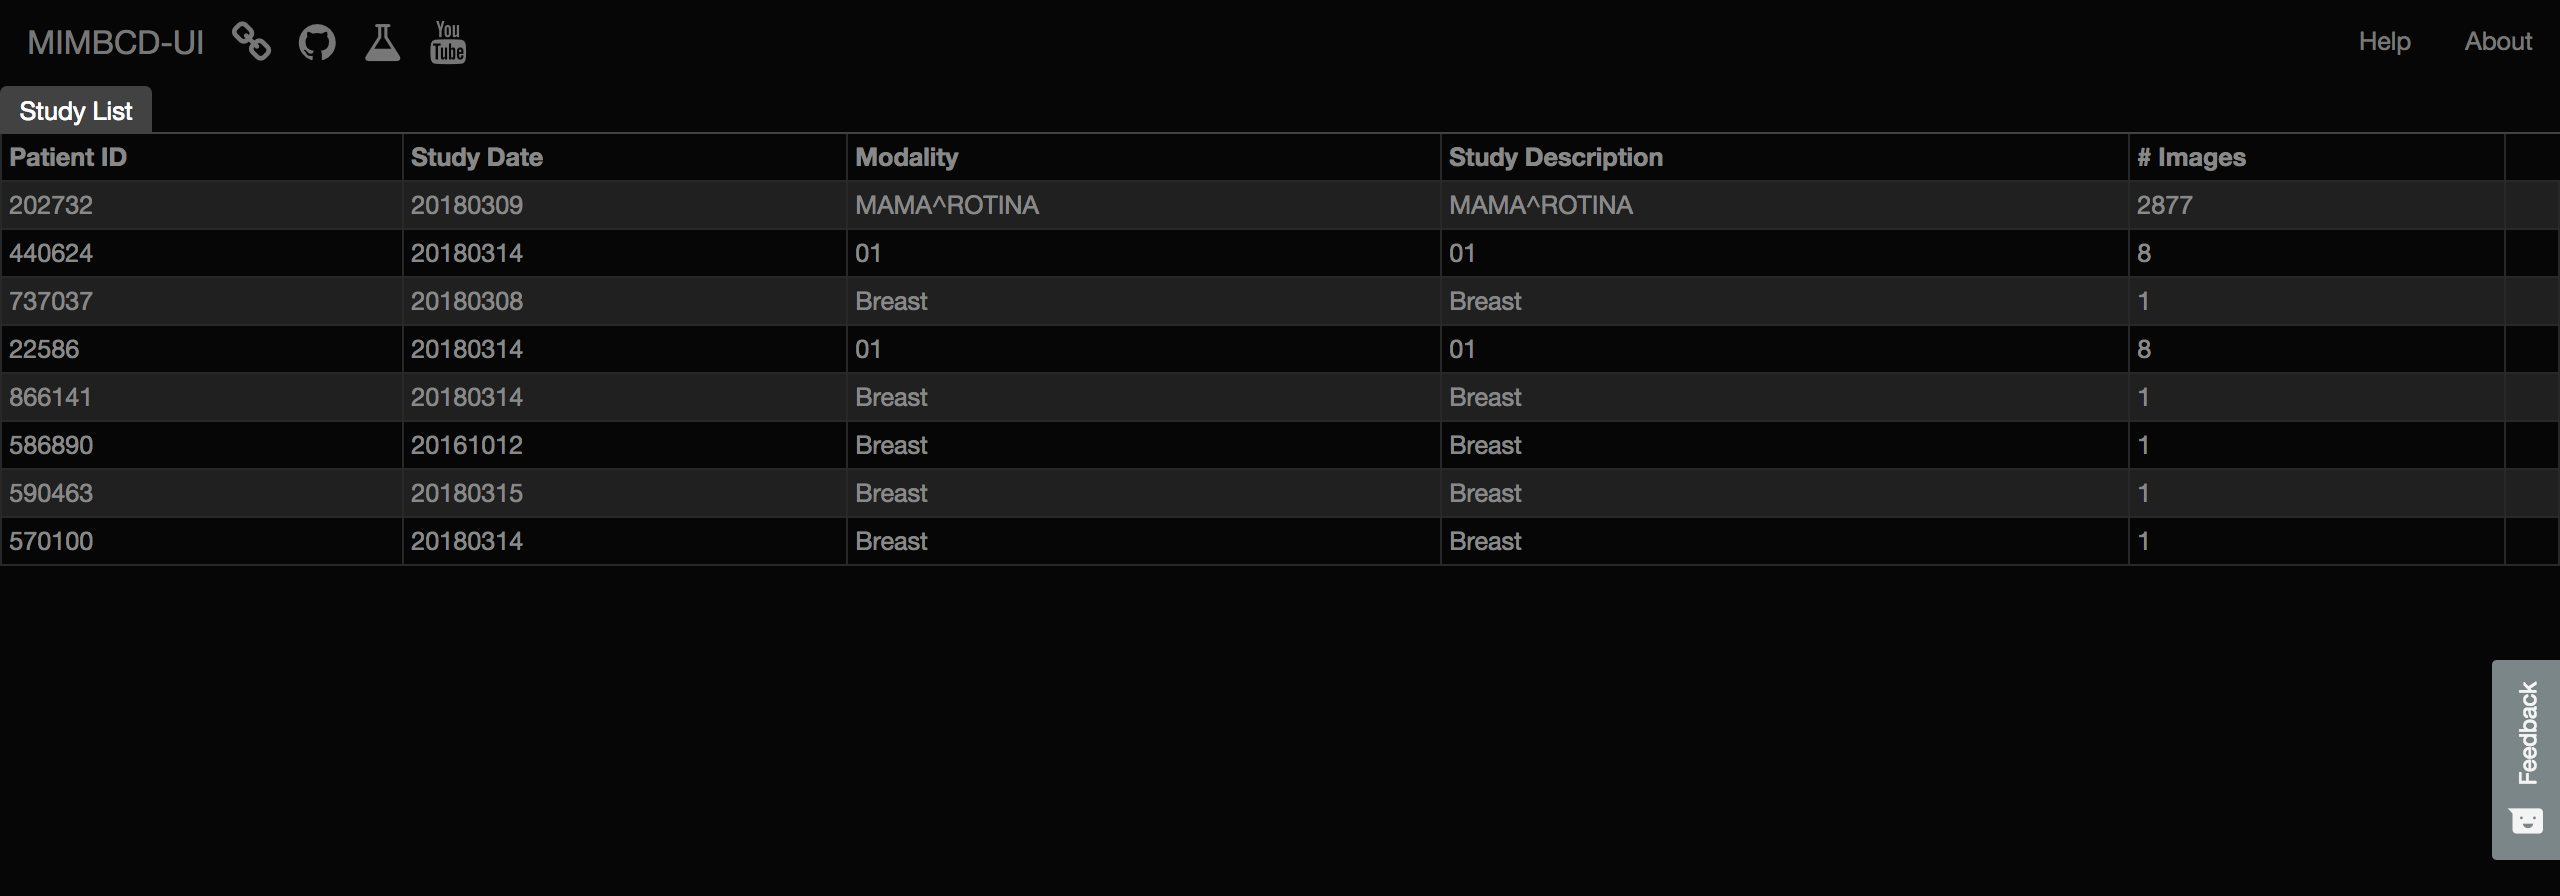
\includegraphics[width=\textwidth]{patient_list}
\caption{List of patients.}
\label{fig:patient_list}
\end{figure}

\hfill

%%%%%%%%%%%%%%%%%%%%%%%%%%%%%%%%%%%%%%%%%%%%%%%%%%%

As we can see in Figure \ref{fig:image_viewer}, it shows the first task in our User Interface (UI), where the patien's breasts are on a small left column. The options are in a short row near of the viewport and described below. We also have the tabs where the user can change the patient. The centre viewport shows the \textbf{DICOM} image, and it can be configured to display a number up to four \textbf{DICOM} images. The viewport has some text information on it (yellow) with the details of the metadata.

\clearpage

%%%%%%%%%%%%%%%%%%%%%%%%%%%%%%%%%%%%%%%%%%%%%%%%%%%

\hfill

\begin{figure}[h]
\centering
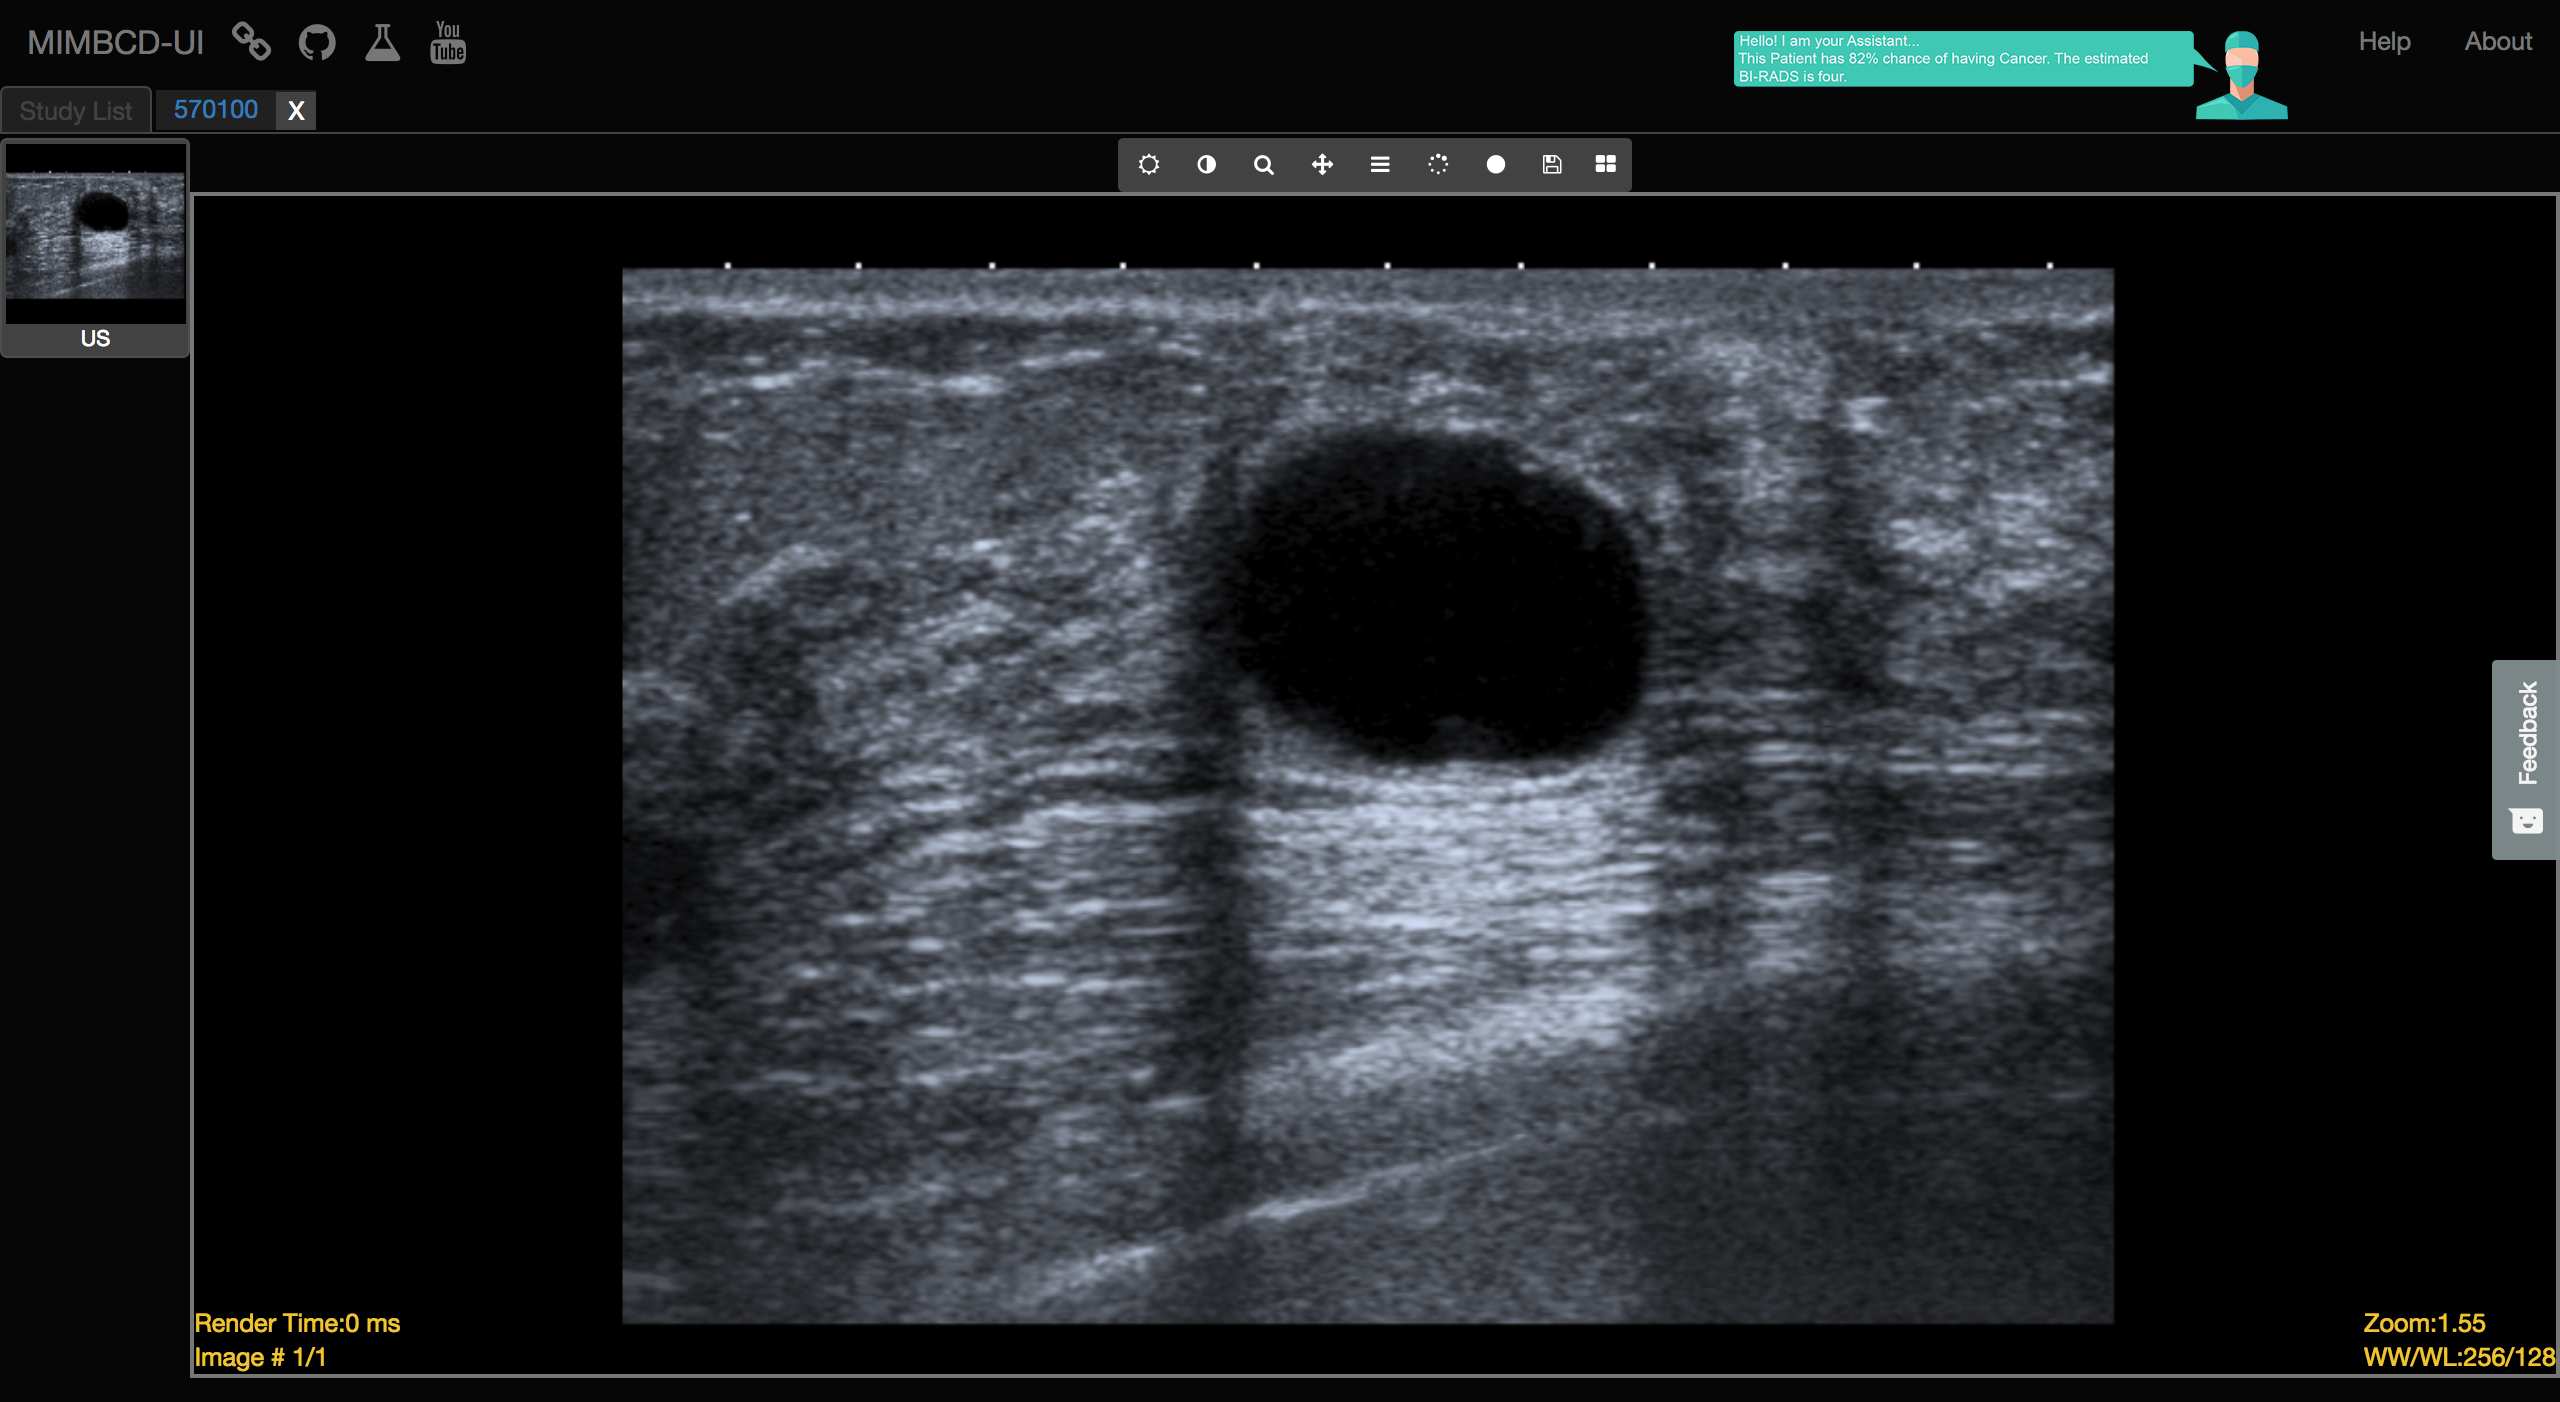
\includegraphics[width=\textwidth]{image_viewer}
\caption{Viewer of the \textbf{DICOM} images.}
\label{fig:image_viewer}
\end{figure}

\hfill

%%%%%%%%%%%%%%%%%%%%%%%%%%%%%%%%%%%%%%%%%%%%%%%%%%%

Manual annotation is adopted by us thanks to Freehand ROI and Probe annotation features, both from CornerstoneJS. According to the CornerstoneJS Library, the user can create an annotation by setting up consecutive landmarks around a Region of Interest (ROI). The markers finish a lesion annotation when it interconnects the historical. Additional features available in our User Interface (UI) includes on-demand increment of the number of landmarks, and throw transformations of the shape of an annotation.

\clearpage

%%%%%%%%%%%%%%%%%%%%%%%%%%%%%%%%%%%%%%%%%%%%%%%%%%%
%                                                 %
%                     SECTION                     %
%                                                 %
%%%%%%%%%%%%%%%%%%%%%%%%%%%%%%%%%%%%%%%%%%%%%%%%%%%

\subsection{User Interactions}

The systems have several buttons (Figure \ref{fig:toolbar}) that allows the user to interact or access to a set of user interface features. Each item of the following list represents each metaphoric icon of Figure \ref{fig:toolbar}.

%%%%%%%%%%%%%%%%%%%%%%%%%%%%%%%%%%%%%%%%%%%%%%%%%%%

\hfill

\begin{figure}[h]
\centering

\includegraphics[width=\textwidth]{toolbar}
\caption{Toolbar of the System available features.}
\label{fig:toolbar}
\end{figure}

\hfill

%%%%%%%%%%%%%%%%%%%%%%%%%%%%%%%%%%%%%%%%%%%%%%%%%%%

\hfill

The buttons are (from left to right of Figure \ref{fig:toolbar}) as follows:

\hfill

\begin{itemize}
\item WW/WC
\item Invert
\item Zoom
\item Pan
\item Stack Scroll
\item Freehand
\item Probe (Deactivated)
\item Save
\item Window Controller
\end{itemize}

\hfill

\clearpage

%%%%%%%%%%%%%%%%%%%%%%%%%%%%%%%%%%%%%%%%%%%%%%%%%%%
%                                                 %
%                     SECTION                     %
%                                                 %
%%%%%%%%%%%%%%%%%%%%%%%%%%%%%%%%%%%%%%%%%%%%%%%%%%%

\subsection{Usability Evaluation Technique}

Usability and functionality are the significant elements which can significantly affect the performance of a medical system. While some prior studies \cite{Calisto:2017:TTM:3132272.3134111} have investigated the functionality of healthcare systems, the usability issue has mostly been overlooked in the existing Health Informatics (HI) literature regarding Human-Computer Interaction (HCI).

The following Table \ref{table:key_questions} is presenting six evaluation questions to have in mind during evaluation. The purpose of this questions is to facilitate systematic user studies in a clinical environment and support the identification of usability problems. The proposed issues involve various aspects of workload combined with either need for satisfaction or division of attention.

\begin{table}[h]
\centering
\label{table:key_questions}
\begin{tabular}{l|l}
Number & Issues of Content Key Questions                    \\ \hline
1      & How do you perceive this activity?                 \\
2      & Could it be done in a more intuitive way?          \\
3      & What are the consequences?                         \\
4      & Why did you do as you did with this activity?      \\
5      & Is this activity relevant for you?                 \\
6      & Could you suggest another way to do this activity?
\end{tabular}
\caption{Usability Evaluation Questions}
\end{table}

The influence of perceived activity \cite{flavian2006role} is an important variable for our empirical analysis. In fact, the trust of the user increases when the user perceived that the system is usable and that there will be a consequent increase of the clinician trust in our system. This arguments explains the first question, the \textit{How do you perceive this activity?} question. For the second question, the \textit{Could it be done in a more intuitive way?} question, we aim to conclude if there is some solution for a more intuitive way of perceive the activity. Third, we intend to filter possible consequences of the clinician workflow by asking \textit{What are the consequences?} directly to the clinician. The fourth question, underlines the reasons why the clinician did that way, with the question \textit{Why did you do as you did with this activity?} we can understand the process of achieving the activity goal and the clinician's interpretation of it. On the fifth question, where we ask \textit{Is this activity relevant for you?}, we aim to understand the potential relevance of our system to the clinician. Last but not least, the six question is present to give the clinician opportunity to suggest improvements, reflecting the reasons why we ask the \textit{Could you suggest another way to do this activity?} question.

To conclude this section, by doing this questions, we aim to support our user studies by giving our users, the clinicians, the opportunity of improving our empirical analysis regarding user's \textit{open answers}. However, the results should be treated with caution. Several bias exists since we are doing here an ambiguous approach.

\clearpage